\documentclass[portrait,a0,final]{a0poster}

\usepackage[utf8]{inputenc}
\usepackage[T1]{fontenc}
\usepackage{lmodern}
\usepackage{multicol}
\usepackage{graphicx}
\usepackage{xcolor}
\usepackage[most]{tcolorbox}
\usepackage{amsmath,amssymb}
\usepackage{booktabs}
\usepackage{array}
\usepackage{enumitem}
\usepackage{microtype}

\setlength{\columnsep}{1.6cm}
\setlength{\columnseprule}{0pt}
\setlength{\parindent}{0pt}
\setlength{\parskip}{0.4em}

% Palette inspired by the conspiracy-detection example (greens)
\definecolor{accent}{RGB}{102,153,102}
\definecolor{accentlight}{RGB}{210,235,212}
\definecolor{accentbg}{RGB}{233,245,233}

\newcounter{secnum}
\newtcolorbox{secbox}[1]{%
  enhanced,
  colback=white,
  colframe=accent,
  boxrule=1.4pt,
  arc=4mm,
  left=14pt,right=14pt,top=10pt,bottom=12pt,
  title={\stepcounter{secnum}\thesecnum.~~#1},
  coltitle=black,
  colbacktitle=accentlight,
  fonttitle=\LARGE\bfseries,
  titlerule=0pt,
  toptitle=8pt,bottomtitle=8pt,
  lefttitle=18pt,
  before skip=10pt,
  after skip=10pt,
}

\begin{document}
\thispagestyle{empty}

% ============== HEADER ==============
\noindent
\begin{minipage}[c]{0.78\linewidth}
  {\fontsize{72}{82}\selectfont\bfseries Continual Learning with O-LoRA:\\[0.15em]
   Orthogonal Low-Rank Adapters for Sequential Tasks\par}
  \vspace{0.7cm}
  {\Large Alex Birsan, Radu Savin\quad\textit{coordinator: TBD}\par}
  \vspace{0.25cm}
  {\large University of Bucharest, Romania\par}
\end{minipage}\hfill
\begin{minipage}[c]{0.20\linewidth}
  \begin{flushright}
    \fbox{\parbox[c][4.2cm][c]{6.5cm}{\centering\Large\bfseries University\\ of Bucharest}}
  \end{flushright}
\end{minipage}

\vspace{0.6cm}
{\color{accent}\rule{\linewidth}{3pt}}
\vspace{0.4cm}

% ============== BODY ==============
\begin{multicols}{2}

% ---------- 1 ----------
\begin{secbox}{Introduction}
\large
Continual learning requires a model to sequentially acquire knowledge across multiple tasks
without forgetting what it previously learned. A common challenge is \textbf{catastrophic forgetting},
where adapting to a new task overwrites representations built for earlier ones.

When parameter-efficient methods such as \textbf{LoRA} are applied in this setting, the low-rank
adapter matrices trained on successive tasks tend to occupy overlapping subspaces, causing
destructive interference. \textbf{O-LoRA} addresses this by imposing an orthogonality constraint
on the $A$ matrices of each new task adapter with respect to all previously learned ones,
ensuring each task projects inputs into a distinct region of the low-rank latent space and thereby
limiting the interference that drives forgetting.
\end{secbox}

% ---------- 2 ----------
\begin{secbox}{Dataset and Preprocessing}
\large
Models are evaluated on a fixed sequence of four text classification tasks:
\begin{itemize}[leftmargin=1.2em,topsep=2pt,itemsep=1pt]
  \item \textbf{AG News} -- 4-class news topic classification
  \item \textbf{Amazon Polarity} -- binary sentiment classification
  \item \textbf{DBpedia 14} -- 14-class Wikipedia topic classification
  \item \textbf{Yahoo Answers Topics} -- 10-class question topics
\end{itemize}
Each task is trained on independently, with no replay of prior task data.

Samples follow the instruction tuning paradigm:
\begin{tcolorbox}[colback=accentbg,colframe=accent,arc=2mm,boxrule=0.5pt,
                  left=8pt,right=8pt,top=4pt,bottom=4pt]
\ttfamily\small \{task instruction\}\textbackslash n\\
Option: \{comma-separated label names\}\textbackslash n\\
\{input text\}\textbackslash n\\
Answer:
\end{tcolorbox}
Only the input text is truncated when the sequence exceeds the maximum length. Cross-entropy
loss is computed only on the label token; at evaluation the predicted label is the candidate
label token with maximum logit at the position before \texttt{Answer}.
\end{secbox}

% ---------- 3 ----------
\begin{secbox}{Model and Experimental Setup}
\large
\textbf{Backbone:} Qwen2.5-1.5B.\\
\textbf{LoRA adapters:} rank $r=8$, scaling $\alpha=32$, dropout $0.1$, applied to the
query and value projections of every attention layer.\\
\textbf{Optimisation:} 1 epoch / task, learning rate $10^{-3}$, batch size $8$.

\textbf{Compared methods:}
\begin{itemize}[leftmargin=1.2em,topsep=2pt,itemsep=1pt]
  \item \textbf{IncLoRA} -- interference-free upper bound: a separate adapter trained
        and frozen for each task ($\text{BWT}=0$ by construction).
  \item \textbf{O-LoRA} -- a single cumulative adapter penalising overlap between the
        new task's $A$ matrix and all previously learned ones via an orthogonal
        regularisation term weighted by $\lambda_1 \in [0.2,0.3]$.
\end{itemize}
\end{secbox}

% ---------- 4 ----------
\begin{secbox}{Orthogonal Regularisation}
\large
For task $t$ with adapter $\Delta W_t = B_t A_t$, the training loss combines the
classification term with a pairwise orthogonality penalty between the current
$A_t$ and every \emph{frozen} previous $A_i$:
\[
\mathcal{L}_t \;=\; \mathcal{L}_{\mathrm{CE}}(A_t,B_t)
\;+\; \lambda_1 \!\!\sum_{i<t}\bigl\lVert A_t A_i^{\!\top}\bigr\rVert_F^{2}
\]
The penalty drives the row-spaces of successive $A$ matrices into mutually
orthogonal directions, so each new task projects inputs into a region of the
low-rank latent space that does not overlap with prior tasks.
Crucially, \textbf{no constraint is applied to the $B$ matrices}.
\end{secbox}

% ---------- 5 ----------
\begin{secbox}{Results}
\large
\textbf{IncLoRA baseline (no forgetting by design):}\par\smallskip
\begin{center}\normalsize
\begin{tabular}{lc}
\toprule
\textbf{Task} & \textbf{Accuracy}\\
\midrule
AG News              & 0.854\\
Amazon Polarity      & 0.956\\
DBpedia 14           & 0.972\\
Yahoo Answers Topics & 0.640\\
\bottomrule
\end{tabular}
\end{center}

\smallskip
\textbf{O-LoRA -- summary metrics:}\par\smallskip
\begin{center}\normalsize
\begin{tabular}{lcccc}
\toprule
\textbf{Run} & \textbf{Samples / task} & $\boldsymbol{\lambda_1}$ & \textbf{Avg Acc} & \textbf{BWT}\\
\midrule
Short             & 500/500/500/500     & 0.3 & 0.846 & $-0.032$\\
2h                & 500/650/1850/1300   & 0.2 & 0.799 & $-0.091$\\
Full ($\sim$50\%) & 2100/2700/7500/5300 & 0.3 & 0.654 & $-0.268$\\
\bottomrule
\end{tabular}
\end{center}

\smallskip
\textbf{Per-task accuracy: initial $\rightarrow$ final:}\par\smallskip
\begin{center}\small
\begin{tabular}{lccc}
\toprule
\textbf{Task} & \textbf{Short} & \textbf{2h} & \textbf{Full ($\sim$50\%)}\\
\midrule
AG News        & 0.878$\to$0.825 ($-6\%$)    & 0.842$\to$0.747 ($-11\%$) & 0.887$\to$0.494 ($-44\%$)\\
Amazon Pol.    & 0.956$\to$0.957 ($\sim$0\%) & 0.947$\to$0.915 ($-3\%$)  & 0.905$\to$0.746 ($-18\%$)\\
DBpedia 14     & 0.964$\to$0.919 ($-5\%$)    & 0.979$\to$0.833 ($-15\%$) & 0.980$\to$0.729 ($-26\%$)\\
Yahoo Ans.     & 0.683$\to$0.683 (---)       & 0.702$\to$0.702 (---)     & 0.649$\to$0.649 (---)\\
\bottomrule
\end{tabular}
\end{center}

\smallskip
Average accuracy and BWT both \textbf{degrade as the number of training samples grows},
even though more data improves \emph{initial} per-task accuracy. The short run is
competitive with IncLoRA with very little forgetting; at $\sim$50\% of the paper's training
scale, BWT collapses to $-0.268$, with AG News losing over $44\%$ of its accuracy.
\end{secbox}

% ---------- 5 ----------
\begin{secbox}{Impact of Prompt Structure}
\large
Switching to the instruction-tuning format -- which explicitly lists all candidate labels
in every prompt -- had a larger effect than any hyperparameter choice.\par\smallskip
\begin{center}\normalsize
\begin{tabular}{lcc}
\toprule
\textbf{Prompt format} & \textbf{Avg Acc} & \textbf{BWT}\\
\midrule
Old (no label options)      & 0.597 & $-0.344$\\
New (instruction + options) & 0.799 & $-0.091$\\
\bottomrule
\end{tabular}
\end{center}

\smallskip
$+0.20$ in accuracy and $+0.25$ in BWT, with substantially less per-task forgetting. Listing
the candidate labels in every prompt acts as a \textbf{task-specific anchor} -- even as adapter
weights shift, the model can recover the correct output distribution by attending to the label
tokens explicitly present in context, rather than relying purely on the adapted weights to
recall which labels are valid.
\end{secbox}

% ---------- 6 ----------
\begin{secbox}{Orthogonality Analysis}
\large
Three pairwise metrics across task adapter matrices:
\begin{itemize}[leftmargin=1.2em,topsep=2pt,itemsep=1pt]
  \item \textbf{Cosine similarity} -- flat-vector directional alignment; blind to subspace structure.
  \item \textbf{Gram Frobenius norm $/r$} -- $\lVert A_i A_j^\top\rVert_F / r$; the quantity
        directly minimised by O-LoRA's loss term.
  \item \textbf{Max principal angle cosine} -- largest singular value of the normalised
        cross-Gram between orthonormalised bases.
\end{itemize}

\begin{center}
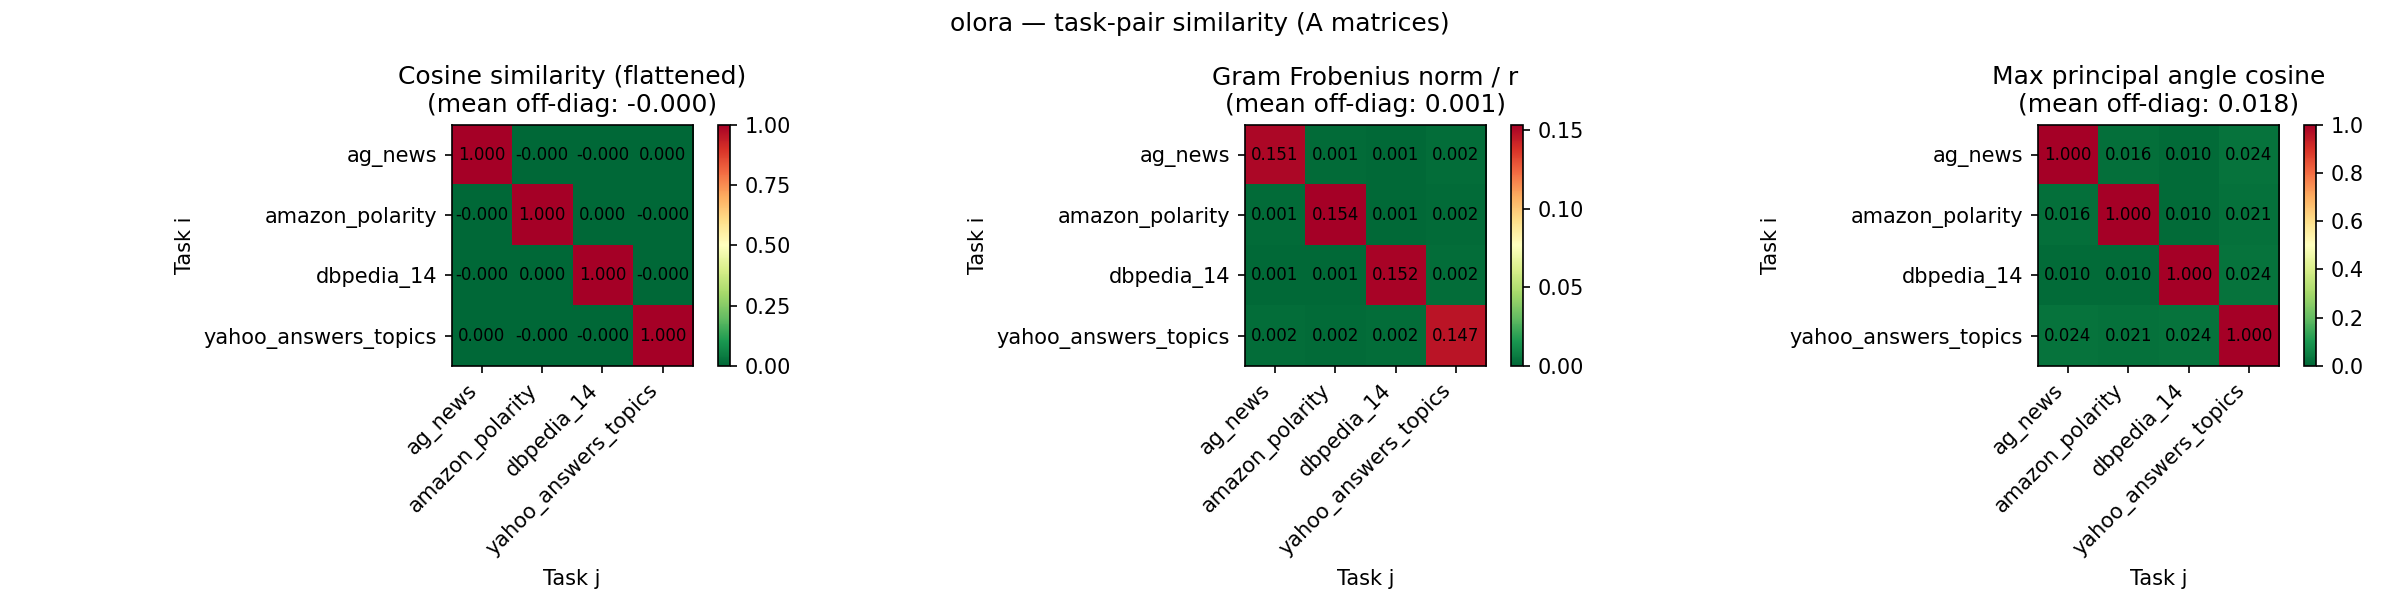
\includegraphics[width=0.96\linewidth]{../results/analysis/olora_task_similarity_A.png}\\[2pt]
{\small Pairwise similarity of $A$ matrices across tasks -- near-zero across all metrics.}
\end{center}

All three metrics show \textbf{near-zero pairwise similarity} across tasks for $A$, even with
$\lambda_1 = 0.2\text{--}0.3$ (lower than the original paper). The constraint is not difficult
to satisfy.

While $B$ matrices are nearly orthogonal as flat vectors (cosine $\sim 0$), their
\textbf{column subspaces share $\sim 30\%$ of their directions} (principal-angle cosine
$\sim 0.29$), and their magnitudes grow proportionally with training steps. Since O-LoRA
imposes no regularisation on $B$, this unconstrained growth is plausibly the primary driver
of forgetting at higher scales.
\end{secbox}

% ---------- 7 ----------
\begin{secbox}{Conclusions}
\large
\begin{itemize}[leftmargin=1.2em,topsep=2pt,itemsep=2pt]
  \item O-LoRA's regulariser keeps $A$ matrices \textbf{geometrically separated} across all
        three metrics, with mild penalties.
  \item Translating geometric separation into reduced forgetting is \textbf{highly sensitive
        to data scale}: near-zero BWT ($-0.032$) at 500 samples/task, sharp collapse
        ($-0.268$) at $\sim$50\% of the paper's scale.
  \item The unregularised $B$ matrices grow in magnitude and share $\sim 30\%$ of column-space
        directions across tasks -- a likely primary driver of forgetting at scale.
  \item \textbf{Prompt structure matters more than hyperparameters}: explicitly listing label
        names yields $+0.20$ accuracy and $+0.25$ BWT.
  \item Non-monotonic recovery of AG News across the 8h run is consistent with unconstrained
        $B$ matrices coincidentally cancelling each other's interference at intermediate
        steps, rather than structured preservation of past knowledge.
\end{itemize}
\end{secbox}

% ---------- References ----------
\begin{secbox}{References}
\normalsize
\begin{enumerate}[leftmargin=1.6em,topsep=2pt,itemsep=2pt,label={[\arabic*]}]
  \item Wang \emph{et al.} \emph{Orthogonal Subspace Learning for Language Model
        Continual Learning.} EMNLP Findings, 2023.
  \item Hu \emph{et al.} \emph{LoRA: Low-Rank Adaptation of Large Language Models.}
        ICLR, 2022.
  \item Qwen Team. \emph{Qwen2.5 Technical Report.} 2024.
  \item Zhang \emph{et al.} \emph{Character-level Convolutional Networks for Text
        Classification (AG News, DBpedia, Yahoo).} NeurIPS, 2015.
  \item McAuley \emph{et al.} \emph{Image-based Recommendations on Styles and
        Substitutes (Amazon Polarity).} SIGIR, 2015.
\end{enumerate}
\end{secbox}

\end{multicols}
\end{document}
